\documentclass{article}

\usepackage{amsmath}
\usepackage{amsthm}
\usepackage{algorithmicx}
\usepackage{algpseudocode}
\usepackage{amsfonts}

\usepackage{flushend}
\usepackage{graphicx}
\usepackage{graphics}
\usepackage{url}
\usepackage[table]{xcolor}
\usepackage{xspace}
\usepackage[T2A]{fontenc}

\usepackage{algorithm}
\usepackage[english]{babel}

\usepackage[utf8]{inputenc}
\usepackage[backend=bibtex]{biblatex}

\usepackage{tabularx}

\newcommand{\OM}{\textsc{OneMax}\xspace}
 \newcommand{\J}{\textsc{Jump}\xspace}
\newcommand{\LB}{\textsc{LeftBridge}\xspace}
\newcommand{\RB}{\textsc{RightBridge}\xspace}
\newcommand{\EARL}{\textsc{EA+RL}\xspace}
\newcommand{\RLS}{\textsc{RLS}\xspace}
\newcommand{\OMZM}{\textsc{OneMax+ZeroMax}\xspace}
\newcommand{\XdK}{\textsc{XdivK}\xspace}

\newtheorem{theorem}{Theorem}
\newtheorem{lemma}{Lemma}
\newtheorem{definition}{Definition}
\newtheorem{corollary}{Corollary}
\addbibresource{bibliography.bib}
\allowdisplaybreaks

\begin{document}

\textit{Note: since I was advsed not to use $\lambda$ as a mutation rate, I use $\alpha$ for this.}

 \section{Applying Our Methods to Fast Evolutionary Algorithm}

For Farst Evolutionary algorithm we have a following transition probabilities from state $i$ to state $j:$

\begin{align*}
  p_{i \to j} = \sum\limits_{\alpha = 1}^{n / 2} C_{n / 2}^\beta \alpha^{-\beta} p_i^j(\alpha),
\end{align*}

Where $p_i^j(\alpha)$ is a probability of transition from state $i$ to state $j$ if the mutation rate is $\alpha$ and $C_{n / 2}^{\beta} = \left(\sum\limits_{\alpha = 1}^{n / 2} \alpha^{-\beta}\right)^{-1}$ is a normalization constant. Notice that $p_i^k(\alpha) = \left(\frac{\alpha}{n}\right)^{k - i} \left(1 - \frac{\alpha}{n}\right)^{n - k + i}.$
Now we introduce and pove two lemmas that are similar to the $(1+1)$-ES with fixed mutation rate.

\begin{lemma}
  $p_{i \to j} \binom{n}{k - i} = p_{j \to i} \binom{n}{k - j}$
\end{lemma}

\begin{proof}
\begin{align*}
  p_{i \to j} \binom{n}{k - i} &= \sum\limits_{\alpha = 1}^{n / 2} C_{n / 2}^\beta \alpha^{-\beta} \binom{n}{k - i} p_i^j(\alpha) \\
  &= \sum\limits_{\alpha = 1}^{n / 2} C_{n / 2}^\beta \alpha^{-\beta} \binom{n}{k - j} p_j^i(\alpha) = p_{j \to i} \binom{n}{k - j}
\end{align*}
\end{proof}

 \begin{lemma}
   For Fast Evolutionary Algorithm we have stationary conditional distribution $\rho^*$ such that $\rho_i^* \sim (1 - p_{i \to k}) \binom{n}{k - i}.$
 \end{lemma}
\begin{proof}
  Let the conditional distribution on iteration $t$ be $\rho(t) = \rho^*.$ Also let $C = \left(\sum\limits_{i = 0}^{k - 1} (1 - p_{i \to k}) \binom{n}{k - i}\right)^{-1}$ be a normalization constant. Then

  \begin{align*}
    \rho_i(t + 1) &= \sum\limits_{j = 0}^{k - 1} \frac{p_{j \to i}}{1 - p_{j \to k}} C(1 - p_{j \to k}) \binom{n}{n - j} \\
                  &= \sum\limits_{j = 0}^{k - 1} \frac{p_{i \to j}}{1 - p_{i \to k}} C(1 - p_{i \to k}) \binom{n}{n - i} \\
                  &= \rho_i(t) \sum\limits_{j = 0}^{k - 1} \frac{p_{i \to j}}{1 - p_{i \to k}} = \rho_i(t).
  \end{align*}
\end{proof}

We obtained the expression for the conditional stationary distribution for Fast Evolutionary Algorithm such that every element of this distribution differs form the elements of the stationary conditional distribution for $(1+1)$-ES with fixed mutation rate only by factor $(1 + o(1)).$ So we can use the same arguments that runtime will not differ more then by factor $(1 + o(1))$ from runtime with initial distribution equal to the stationary conditional distribution that is $1 / p_{end}^*$.

\section{Comparation of the Runtimes}

Computation has shown that the expected runtime for the Fast EA is slightly greater than the expected runtime for the fixed mutation rate, but only by a factor not greater than $1.43$ for $n \le 10^4$. Dependence of this factor on $n$ and $k$ is shown in Fig.~\ref{runtimes_over_n} and in Fig.~\ref{runtimes_over_k}. We use $\beta = 2$ for the Fast EA as long as it seems to be most optimal value, which is justified below.

\begin{figure}
  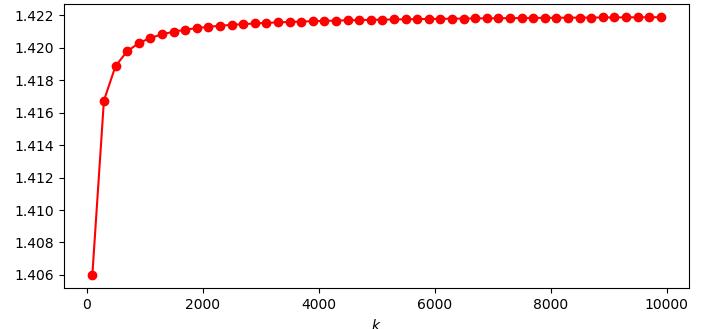
\includegraphics[width=0.8\textwidth]{pic/runtime_ratio_k10.png}
  \caption{Ratio of the expected runtime of the Fast EA to the expected runtime of the $(1 + 1)$-ES with optimal mutation rate for $k = 10$. It does not differ for other values of $k$, so we do not present results for them here.}\label{runtimes_over_n}
\end{figure}


\begin{figure}
  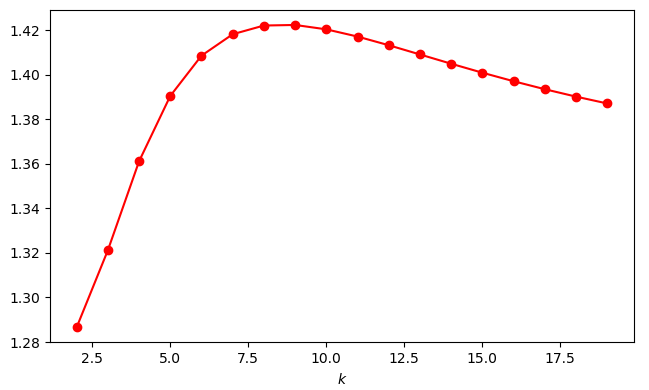
\includegraphics[width=0.8\textwidth]{pic/runtime_ratio_n1000.png}
  \caption{Ratio of the expected runtime of the Fast EA to the expected runtime of the $(1 + 1)$-ES with optimal mutation rate for $n = 1000$.}\label{runtimes_over_k}
\end{figure}

Now let us compare runtimes of the $(1 + 1)$-ES with fixed mutation rate and the Fast EA theoretically. As long as for both of them runtime is $1/p_{end}^*,$ let us only consider $p_{end}^*.$ We will use the following bounds on partial sums of binomial numbers in some equations:

$$\binom{n}{k} \le \sum\limits_{i = 0}^{k - 1} \binom{n}{k - i} \le \binom{n}{k} \frac{n - k + 1}{n - 2k + 1} = \binom{n}{k}(1 + o(1)).$$


Consider $p_{end}^*$ for the fixed mutation rate:

\begin{align*}
  p_{end}^* &= \frac{\sum\limits_{i = 0}^{k - 1}p_i^k (1 - p_i^k) \binom{n}{k - i}}{\sum\limits_{i = 0}^{k - 1}(1 - p_i^k) \binom{n}{k - i}} = \frac{\sum\limits_{i = 0}^{k - 1}p_i^k \binom{n}{k - i}}{\sum\limits_{i = 0}^{k - 1}\binom{n}{k - i}} (1 + o(1)) \\
            &= \frac{\sum\limits_{i = 0}^{k - 1}p_i^k \binom{n}{k - i}}{\binom{n}{k}} (1 + o(1))
\end{align*}

And consider this value for the Fast EA:

\begin{align*}
  p_{end}^* &= \frac{\sum\limits_{i = 0}^{k - 1}p_{i \to k} (1 - p_{i \to k}) \binom{n}{k - i}}{\sum\limits_{i = 0}^{k - 1}(1 - p_{i \to k}) \binom{n}{k - i}} = \frac{\sum\limits_{i = 0}^{k - 1}p_{i \to k} \binom{n}{k - i}}{\sum\limits_{i = 0}^{k - 1}\binom{n}{k - i}} (1 + o(1))\\
            &= \frac{\sum\limits_{i = 0}^{k - 1}p_{i \to k} \binom{n}{k - i}}{\binom{n}{k}} (1 + o(1)) \\
\end{align*}

Consider the numerator:

\begin{align*}
  \sum\limits_{i = 0}^{k - 1}p_{i \to k} \binom{n}{k - i} = \sum\limits_{i = 0}^{k - 1} \binom{n}{k - i} \sum\limits_{\alpha = 1}^{n / 2} C_{n / 2}^\beta \alpha^{-\beta} p_i^k(\alpha) = \sum\limits_{\alpha = 1}^{n / 2} C_{n / 2}^\beta \alpha^{-\beta} \sum\limits_{i = 0}^{k - 1} p_i^k(\alpha)\binom{n}{k - i}
\end{align*}

So it is a convex combination of values that are not greater than the numerator for fixed mutation rate (as long as we consider the optimal one). So the runtime for Fast EA can not be less then runtime for the optimal fixed mutation rate. However how much worse is it?

Consider the numerator for the fixed mutation rate more precisely:

\begin{align*}
  \sum\limits_{i = 0}^{k - 1}p_i^k \binom{n}{k - i} &= \sum\limits_{i = 0}^{k - 1} \binom{n}{k - i} \left(\frac{\alpha}{n}\right)^{k - i}\left(1  - \frac{\alpha}{n}\right)^{n - k + i} \\
  &= (1 + o(1)) e^{-\alpha} \sum\limits_{i = 0}^{k - 1} \frac{n!\alpha^{k - i}}{(k - i)!(n - k + i)!n^{k - i}} \\
  &= (1 + o(1)) e^{-\alpha} \sum\limits_{i = 1}^k \frac{\alpha^i}{i!} \\
  &\le (1 + o(1))e^{-\alpha} (e^\alpha - 1) = (1 + o(1)) (1 - e^{-\alpha}).
\end{align*}

At the same time consider the numerator for the Fast EA:

\begin{align*}
  \sum\limits_{i = 0}^{k - 1}p_{i \to k} \binom{n}{k - i} &= \sum\limits_{i = 0}^{k - 1} \binom{n}{k - i} \frac{\sum\limits_{\alpha = 1}^{n / 2} \alpha^{-\beta} \left(\frac{\alpha}{n}\right)^{k - i} \left(1 - \frac{\alpha}{n}\right)^{n - k + i}}{\sum\limits_{\alpha = 1}^{n / 2} \alpha^{-\beta}} \\
  &= (1 + o(1)) \sum\limits_{i = 0}^{k - 1} \binom{n}{k - i} \frac{1}{n^{k - i}} \frac{\sum\limits_{\alpha = 1}^{+\infty} \alpha^{k - i - \beta} e^{-\alpha}}{\sum\limits_{\alpha = 1}^{n/2} \alpha^{-\beta}} \\
  &= (1 + o(1)) \sum\limits_{i = 0}^{k - 1}\frac{1}{(k - i)!}\frac{\text{Li}_{\beta + i - k}(e^{-1})}{\sum\limits_{\alpha = 1}^{n/2} \alpha^{-\beta}}.
\end{align*}




Here $\text{Li}_s(x)$ is the polylogarithm function.

So, the ratio of the expected runtimes of Fast EA and $(1 + 1)$-EA with optimal mutation rate is not greater than:

\begin{align*}
  \frac{T_{fea}}{T_{opt}} \le \frac{(1 - e^{-\sqrt[k]{k!}})\sum\limits_{\alpha = 1}^{n/2} \alpha^{-\beta}}{\sum\limits_{i = 0}^{k - 1}\frac{\text{Li}_{\beta + i - k}(1/e)}{(k - i)!}}.
\end{align*}

\begin{figure}
  \begin{center}
  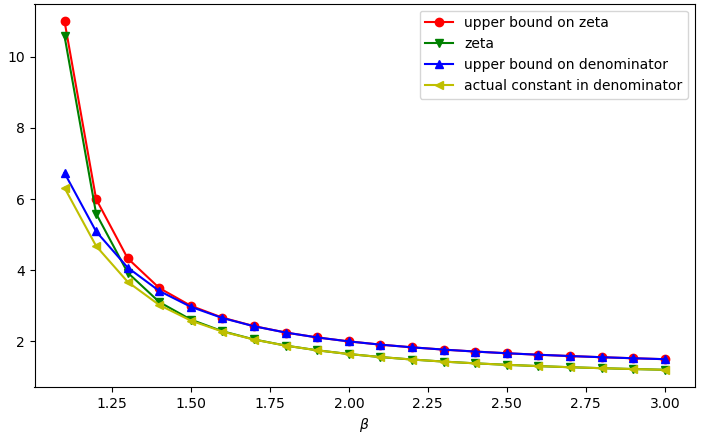
\includegraphics[width=0.8\textwidth]{pic/zeta_small.png}
  \end{center}
  \caption{Computed values for upper bound on Reimann's zeta function upper bound $\beta/(\beta - 1)$, Reimann's zeta function, upper bound on inversed normalization constant $\frac{\beta - (n/2)^{1 -\beta}}{\beta - 1}$ and the inversed normalization constant itself  for $n = 1000.$
  \label{zeta}}
\end{figure}

\subsection{Bounds on Normalization Constant for Heavy-Tailed Mutation}

Obvious solution is to bound normalization constant in the following way:

\begin{align*}
  C_{n/2}^\beta = \frac{1}{\sum\limits_{\alpha = 1}^{+\infty} \alpha^{-\beta}} \ge \frac{1}{\sum\limits_{\alpha = 1}^{+\infty} \alpha^{-\beta}} = \zeta^{-1}(\beta) \ge \frac{\beta - 1}{\beta},
\end{align*}
where $\zeta(\beta)$ is the Reimann's Zeta function. However, this is a rough bound for values of $\beta$ that are close to one, as for such values the series of $\sum\limits_{\alpha = 1}^{+\infty} \alpha^{-\beta}$ converges very slowly.

So we will bound directly the value of $\sum\limits_{\alpha = 1}^{n/2} \alpha^{-\beta}$:

\begin{align*}
  \sum\limits_{\alpha = 1}^{n/2} \alpha^{-\beta} &\le 1^{-\beta} + \sum\limits_{\alpha = 2}^{n/2}\int\limits_{\alpha - 1}^{\alpha} x^{-\beta} dx = 1 + \int\limits_1^{n/2} x^{-\beta} dx \\
  &= 1 - 1/(1 - \beta) + \frac{(n/2)^{1 -\beta}}{1 - \beta}= \frac{\beta- (n/2)^{1 -\beta}}{\beta - 1}.
\end{align*}

And it seems to be quite a precise bound. Computational comparation of zeta function, bound on zeta function, inversed normalization constant and more precise bound on it are shown in Fig.~\ref{zeta}.



\subsection{Polylogarithm}

Obtaining bounds for polylogarithm is more tricky. According to computation, for $s \ge 2$ polylogarithm $\text{Li}_{-s}(1/e)$ is almost equals to the Euler's gamma function $\Gamma(s + 1)$, they differ no more then on $0.5\%$ of their values and this relative defference decreases with growth of $s$. However, I did not find any information about this connection between polylogarithm and Gamma function, despite of there are plenty of different representations of polylogarithm, most of which can be found in~\cite{polylog} (the closest ones to what we need are equations 13.1 and 17.1). Nevertheless we still can obtain quite a good bound.

First, consider case when $s > 1$. If we consider the derivative of $\alpha^s e^{-\alpha},$ we can see that this function is increasing, if $0 < \alpha < s$, and it is decreasing, if $\alpha > s$. So we can say:

\begin{align*}
  \text{Li}_{-s}(1/e) &= \sum\limits_{\alpha = 1}^{+ \infty} \alpha^s e^{-\alpha} = \sum\limits_{\alpha = 1}^{\lfloor s \rfloor} \alpha^s e^{-\alpha} + \sum\limits_{\lfloor s \rfloor + 1}^{+\infty} \alpha^s e^{-\alpha} \\
  &\ge \sum\limits_{\alpha = 1}^{\lfloor s \rfloor} \int\limits_{\alpha - 1}^\alpha x^s e^{-x} dx + \sum\limits_{\lfloor s \rfloor + 1}^{+\infty} \int\limits_\alpha^{\alpha + 1} x^s e^{-x} dx \\
  &\ge \int\limits_0^{+\infty} x^s e^{-x} dx - \int\limits_{\lfloor s \rfloor}^{\lfloor s \rfloor + 1} x^s e^{-x} dx \\
  &\ge \Gamma(s + 1) - (s / e)^s \\
  &\ge \Gamma(s + 1) \left(1 - \sqrt{\frac{1}{2 \pi s}}\right),
\end{align*}
where $\Gamma(s + 1)$ is the Euler's Gamma function and the last inequation is justified by the bounds on Stirling's approximation of the Gamma function.

For $s \le 1$ notice that $\text{Li}_{-s}(1/e)$ is increasing with growth of $s$. So we can tell that $\text{Li}_{-s}(1/e) > \text{Li}_{\lceil-s\rceil}(1/e)$. As long as we cosider only $\beta \le 3$ and thus, $k - i - \beta \ge -2$, we also need to introduce the following constants:

\begin{itemize}
  \item $\text{Li}_0(1/e) = \frac{1}{e - 1} \ge 0.58$
  \item $\text{Li}_1(1/e) = -\ln(1 - 1/e) \ge 0.45$
  \item $\text{Li}_2(1/e) = \sum\limits_{\alpha = 1}^{+\infty} \frac{e^{-\alpha}}{\alpha^2} \ge \frac{1}{e} + \frac{1}{4e^2} \ge 0.4$
\end{itemize}


Now let us consider $\beta \in (1, 2].$ In this case:

\begin{align*}
  \sum\limits_{i = 0}^{k - 1} \frac{\text{Li}_{\beta + i - k}(1/e)}{(k - i)!} &= \text{Li}_{\beta - 1}(1/e) + \text{Li}_{\beta - 2}(1/e) + \sum\limits_{i = 3}^{k} \frac{\text{Li}_{\beta - i}(1/e)}{i!} \\
  & \ge \text{Li}_1(1/e) + \frac{\text{Li}_0(1/e)}{2} + \sum\limits_{i = 3}^{k} \frac{\Gamma(i - 1)\left(1 - \sqrt{\frac{1}{2\pi}}\right)}{i!} \\
  &= -\ln(1 - 1/e) + \frac{1}{2(e - 1)} + \left(1 - \sqrt{\frac{1}{2\pi}}\right) \left(\frac{1}{2} - \frac{1}{k}\right) \\
  &\approx 1.05 - 0.60 / k.
\end{align*}

When $\beta \in (2, 3]$:

\begin{align*}
  \sum\limits_{i = 0}^{k - 1} \frac{\text{Li}_{\beta + i - k}(1/e)}{(k - i)!} &= \text{Li}_{\beta - 1}(1/e) + \text{Li}_{\beta - 2}(1/e) + \text{Li}_{\beta - 3}(1/e) + \sum\limits_{i = 4}^{k} \frac{\text{Li}_{\beta - i}(1/e)}{i!} \\
  & \ge \text{Li}_2(1/e) + \frac{\text{Li}_1(1/e)}{2} + \frac{\text{Li}_0(1/e)}{6} + \sum\limits_{i = 4}^{k} \frac{\Gamma(i - 1)\left(1 - \sqrt{\frac{1}{2\pi}}\right)}{i!} \\
  &= \left(\frac{1}{e} + \frac{1}{4e^2}\right)-\frac{\ln(1 - 1/e)}{2} + \frac{1}{6(e - 1)} + \left(1 - \sqrt{\frac{1}{2\pi}}\right) \frac{1}{2}\left(\frac{1}{6} - \frac{1}{k(k - 1)}\right)
  \\ &\approx 0.78 - \frac{0.30}{k(k - 1)}.
\end{align*}

Notice that if $k = 2$, then we have only two first summands:

\begin{align*}
  \sum\limits_{i = 0}^{1} \frac{\text{Li}_{\beta + i - 2}(1/e)}{(2 - i)!} \ge \text{Li}_2(1/e) + \frac{\text{Li}_1(1/e)}{2} \approx 0.63.
\end{align*}

This bound is less than the bound for $\beta \in (1, 2],$ so we will not use it to compare runtimes.

\subsection{Summing Up the Results}

So, for $(1 + 1)$-ES with the optimal mutation rate we have the following lower bound on rumtime:

\begin{align*}
  T_{fixed} \ge (1 + o(1))\binom{n}{k} \frac{1}{1 - e^{-\sqrt[k]{k!}}}.
\end{align*}

For Fast EA we got the followin upper bound on runtime (I use approximate values here not to make it too heavy):

\begin{align*}
  T_{fea} \le (1 + o(1))\binom{n}{k} \frac{\beta - (n/2)^{1 - \beta}}{\beta - 1} \frac{1}{1.05 - 0.61/k}
\end{align*}

If we use $\beta = 2,$ it maximizes $\frac{\beta - (n/2)^{1 - \beta}}{\beta - 1}.$ We can not use greater values, as we use border fro $\beta \in (1, 2].$

Totally we have:

\begin{align*}
  \frac{T_{fea}}{T_{fixed}} \le (1 + o(1)) \frac{2(1 - e^{-\sqrt[k]{k!}})}{1.05 - 0.61/k}
\end{align*}

This result is not very precise, but you can see its comparation with actual data on Fig.~\ref{comparation_n} and Fig.~\ref{comparation_k}

\begin{figure}
  \begin{center}
    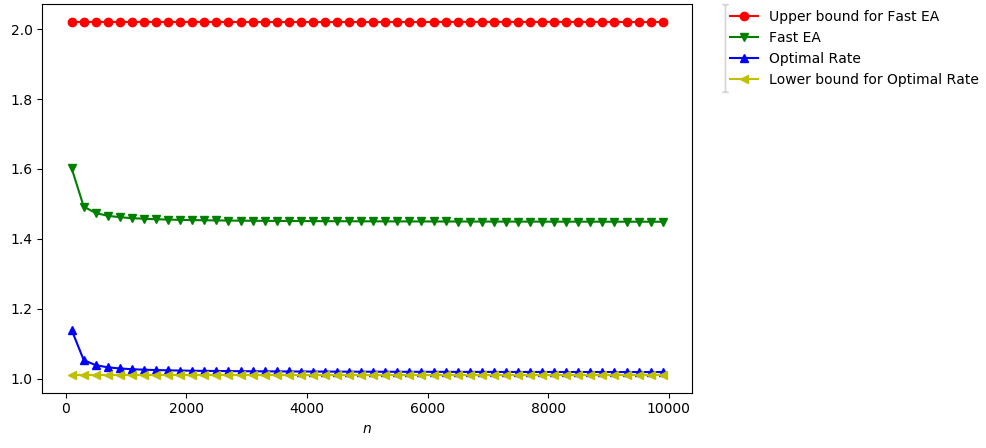
\includegraphics[width=0.8\textwidth]{pic/final_n.png}
  \end{center}
  \caption{Comparation of the ratio of runtimes to $\binom{n}{k}$ for the Fast EA, $(1 + 1)$-ES with optimal mutation rate and for the bounds on these runtimes for $k = 10$.\label{comparation_n}}
\end{figure}


\begin{figure}
  \begin{center}
    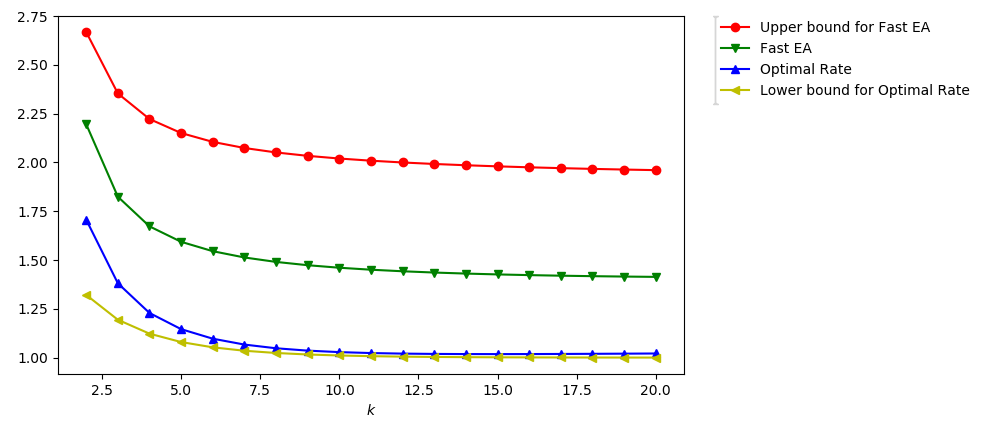
\includegraphics[width=0.8\textwidth]{pic/final_k.png}
  \end{center}
  \caption{Comparation of the ratio of runtimes to $\binom{n}{k}$ for the Fast EA, $(1 + 1)$-ES with optimal mutation rate and for the bounds on these runtimes for $n = 1000$.\label{comparation_k}}
\end{figure}

\printbibliography
\end{document}
